%%%%%%%%%%%%%%%%%%%%%%%%%%%%%%%%%%%%%%%%%%%%%%%%%%
%Proyecto: Ejemplo de latex
%Colaboradores: Ljoh
%Fecha: 26 sep 2020
%%%%%%%%%%%%%%%%%%%%%%%%%%%%%%%%%%%%%%%%%%%%%%%%%%%

%================================================================
%				Tipo de documeto
%================================================================
\documentclass[12pt]{article}
%10pt,12pt twocolumns
%================================================================
%					Preambulo
%================================================================
\usepackage{lmodern}
\usepackage[utf8]{inputenc}
\usepackage[T1]{fontenc}
\usepackage[spanish,activeacute]{babel}

\usepackage{multicol}
\usepackage{enumerate}
\usepackage{enumitem}
\usepackage{booktabs}
\usepackage{tabularx, makecell}


\usepackage{lipsum}
\usepackage{float}

\usepackage{mathtools}
\usepackage{amssymb, amsmath, amsbsy} % simbolitos
%\usepackage{upgreek} % para poner letras griegas sin cursiva
\usepackage{cancel} % para tachar
\usepackage{mathdots} % para el comando \iddots
\usepackage{mathrsfs} % para formato de letra
\usepackage{stackrel} % para el comando \stackbin
\usepackage{multirow} % para las tablas
%\usepackage[fleqn]{amsmath}
\usepackage{nccmath}
\usepackage{multicol} %Texto en multiples columnas

\usepackage{graphicx} % figuras
\usepackage{subfigure} % subfiguras

%Circuitos
\usepackage{tikz,pgfplots}
\usepackage[europeanresistors,americaninductors]{circuitikz}

\usetikzlibrary{calc}
\usetikzlibrary{patterns}

\ctikzset{bipoles/thickness=1}%Grosor de los elementos pasivos
\ctikzset{bipoles/length=1.2cm}%Longitud de los elementos pasivos
\tikzstyle{every node}=[font=\normalsize] %tamaño de etiquetas
\tikzstyle{every path}=[line width=1.25pt, line cap=round, line join=round] %caracteristicas de la linea union


\usepackage{wasysym}


\usepackage{xcolor}

%================================================================
%					Comandos
%================================================================
\definecolor{ColorRespuesta}{RGB}{12,79,182}
\newcommand{\Respuesta}[1]{\textcolor{ColorRespuesta}{#1}}
\newcommand{\derivada}[2]{\displaystyle{\frac{d#1}{d#2}}}
%================================================================
%					Margenes
%================================================================
\setlength{\textwidth}{170mm}%Ancho de Texto
\setlength{\textheight}{230mm}%Largo del Texto
\setlength{\oddsidemargin}{-5mm}%Margen de pagunas impares
\setlength{\evensidemargin}{5mm}%Margen de páginas pares
								%-para documentos tipo book-
\setlength{\topmargin}{-20mm}%Margeb Superior

%================================================================
%				  Datos del Autor
%================================================================
\title{Capitulo A}
\author{Luis J Olguín}
\date{\today}
%================================================================
%					Documento
%================================================================


\begin{document}

\maketitle

	\begin{figure}
		\centering
		\tikz \draw[thick,rounded corners=8pt]
			(0,0) -- (0,2) -- (1,3.25) -- (2,2) -- (2,0) -- (0,2) -- (2,2) -- (0,0) -- (2,0);

		\caption{Casita de una linea}
		\label{FIG:Casa-una-linea}

	\end{figure}
	
	\begin{figure}[htb]%h: here, t: top al principio de la pagina, b: al final de la página, !
		\centering %alineación 
		%%Figura*********************************************************
							%Simbologia europea o ameriaca, escala de la figura
		\begin{circuitikz}[american,scale=1.5, transform shape]
		    \draw (0,0) to [short,-*](0,0); %punto de voltaje -
			\draw (0,2) to [short,*-](0,2); %punto de voltaje +
			\draw (0,2) to [sV=$V_{i}$](0,0); %Etiqueta voltaje
			%filtro LCL
			\draw (0,2) to [L,l=$L_{1}$,f=$i_{L_1}$](3.1,2); %Inductacia L1 y corriente i1
			%\draw (3.1,2) to [L,l=$L_{2}$,f=$i_{g}$](5.1,2); %Inductacia L2 y corriente ig
			%\draw (5.1,2) to [short,-*](5.6,2); %punto de voltaje -
			%\draw (5.6,0) to [short,*-](3.1,0); %punto de voltaje +
			\draw (3.1,0) to [C, l=$C_{f}$, f=$i_{C_{f}}$](3.1,2); %Inductacia L2 y corriente ig
			%\draw (0,0) to [short,-](3.1,0); %punto de voltaje +
			\draw  (3.1,0) to [R,l=$R_1$,f=$i_{R_{1}}$](0,0);
			%\draw (5.6,2) to [open,v=$V_{o}$](5.6,0); %Etiqueta voltaje

		\end{circuitikz}
		%%************************************************************Final Figura
		\caption{Circuito RC}
		\label{FIG:CircuitoRC}
	\end{figure}
	



	Analisis del Circuito RC en \LaTeX{} de la figura \ref{FIG:CircuitoRC}

	$V(t)=A\sin(\omega t)$

	$V_{C_1}=\displaystyle{\frac{q(t)}{C_1}} $

	\begin{multicols}{2}
		Hola que ta??

		\begin{equation}
			\begin{split}
			V_{R_1}&=iR_1=\derivada{q(t)}{t}R_1\\
			&=iR_1=\derivada{q(t)}{t}R_1
			\end{split}
		\end{equation}
		$
		\begin{array}{ll}
			V_{R_1}&=iR_1=\derivada{q(t)}{t}R_1\\
			&=iR_1=\derivada{q(t)}{t}R_1
		\end{array}
		$

		Lorem ipsum dolor sit amet, consectetur adipisicing elit, 
		sed do eiusmod tempor incididunt ut labore et dolore magna 
		aliqua. Ut enim ad minim veniam, quis nostrud exercitation 
		ullamco laboris nisi ut aliquip ex ea commodo consequat. 
		Duis aute irure dolor in reprehenderit in voluptate velit 
		esse cillum dolore eu fugiat nulla pariatur. Excepteur sint 
		occaecat cupidatat non proident, sunt in culpa qui officia 
		deserunt mollit anim id est laborum.
		
		\begin{figure}[H]
			\centering
			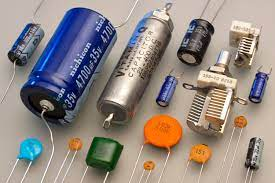
\includegraphics[width=4cm, height=6cm]{imagenes/capacitores.jpg}
			\caption{Tipos de Capacitores}
			\label{FIG:Capacitores}
		\end{figure}

		Lorem ipsum dolor sit amet, consectetur adipisicing elit, sed 
		do eiusmod tempor incididunt ut labore et dolore magna aliqua. 
		Ut enim ad minim veniam, quis nostrud exercitation ullamco 
		laboris nisi ut aliquip ex ea commodo consequat. Duis aute irure 
		dolor in reprehenderit in voluptate velit esse cillum dolore eu 
		fugiat nulla pariatur. Excepteur sint occaecat cupidatat non 
		proident, sunt in culpa qui officia deserunt mollit anim id 
		est laborum.
		
		\begin{figure}[H]
			\centering
			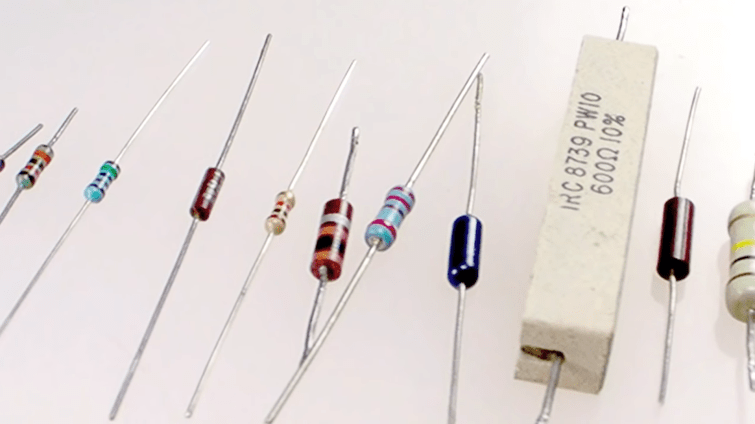
\includegraphics[height=4cm]{imagenes/resistencias.png}
			\caption{Tipos de Resistores}
			\label{FIG:Resistores}
		\end{figure}
		Lorem ipsum dolor sit amet, consectetur adipisicing elit, sed 
		do eiusmod tempor incididunt ut labore et dolore magna aliqua. 
		Ut enim ad minim veniam, quis nostrud exercitation ullamco 
		laboris nisi ut aliquip ex ea commodo consequat. Duis aute irure 
		dolor in reprehenderit in voluptate velit esse cillum dolore eu 
		fugiat nulla pariatur. Excepteur sint occaecat cupidatat non 
		proident, sunt in culpa qui officia deserunt mollit anim id 
		est laborum.
		
	\end{multicols}

	
	\begin{figure}[b!]
		\centering
		\begin{tikzpicture}
		    \begin{axis}[domain=0:1,legend pos=outer north east]
		    \addplot {sin(deg(x))}; 
		    \addplot {cos(deg(x))}; 
		    \addplot {x^2};
		    \legend{$\sin(x)$,$\cos(x)$,$x^2$}
		    \end{axis}
		\end{tikzpicture}
		\caption{Grafica de funciones}
		\label{FIG:Grafica-de-Senos}
	\end{figure}

	
	
	\begin{figure}
		\centering
		\begin{tikzpicture}
			\draw (-1.5,0) -- (1.5,0);
			\draw (0,-1.5) -- (0,1.5);
			\draw (-1,0) .. controls (-1,0.555) and (-0.555,1) .. (0,1)
			.. controls (0.555,1) and (1,0.555) .. (1,0);
			\end{tikzpicture}

		\caption{Medio Circulo}
		\label{FIG:Medio-circulo}

	\end{figure}
	$$
	X=12,\ Y=13;
	S=2X+Y
	S=2(12)+13
	$$
    %Casos de uso de Inicio de Sesión

\end{document}
